\section{Technical overview}
\label{sec:katharatechnicaloverview}

In Kathará's original announcement's paper~\cite{kathara}, the described technical infrastructure of the program, which can easily be confirmed by consulting the available Python source code,\footnote{\url{https://github.com/KatharaFramework/Kathara}}, clearly states the basic design decision that follows the choosing of lightweight containers via Docker: every node in the topology is a Docker container.
Kathará, therefore, works as an orchestrator of containers, the same way that Docker's own Compose\footnote{\textquote{Compose is a tool for defining and running multi-container Docker applications \ldots\ with a single command, you create and start all the services from your configuration.}~\url{https://docs.docker.com/compose/}} is.
The difference is that, while Docker Compose exposes a limited set of network parameterization, given that its purpose is to handle the combination of different application-level services running in containers that must be able to exchange IP traffic between each other, Kathará uses lower-level primitives exposed by Docker itself to setup the containers' virtual interfaces and hook them up to virtual collision domains which serve as a shared medium between any number of nodes, and therefore constitute links or hubs in a topology.

% Figure fig:kathara-architecture-paper
\begin{figure}
  \centering
  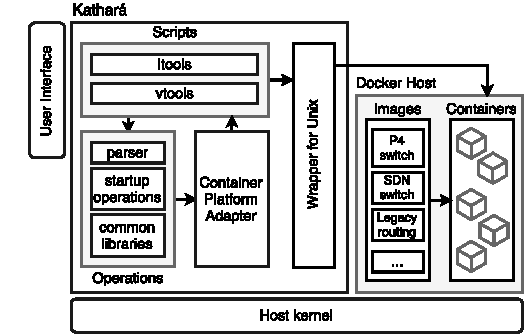
\includegraphics[width=0.8\textwidth]{kathara-architecture-paper}
  \caption{The diagram where Kathara's authors present its architecture}
  \label{fig:kathara-architecture-paper}
\end{figure}


Kathará also leverages the notion of Docker images, available via Docker Hub or just setup locally on the user's Docker installation, both for separating the functionality (and ``role'') that different kinds of nodes may have on a lab (from being a traditional router to an OpenFlow switch, or an end-host running a RDBMS). % TODO add RDBMS to the acronyms

% end of section katharatechnicaloverview
